% $Id: template.tex 11 2007-04-03 22:25:53Z jpeltier $

\documentclass{vgtc}                          % final (conference style)
%\documentclass[review]{vgtc}                 % review
%\documentclass[widereview]{vgtc}             % wide-spaced review
%\documentclass[preprint]{vgtc}               % preprint
%\documentclass[electronic]{vgtc}             % electronic version

%% Uncomment one of the lines above depending on where your paper is
%% in the conference process. ``review'' and ``widereview'' are for review
%% submission, ``preprint'' is for pre-publication, and the final version
%% doesn't use a specific qualifier. Further, ``electronic'' includes
%% hyperreferences for more convenient online viewing.

%% Please use one of the ``review'' options in combination with the
%% assigned online id (see below) ONLY if your paper uses a double blind
%% review process. Some conferences, like IEEE Vis and InfoVis, have NOT
%% in the past.

%% Figures should be in CMYK or Grey scale format, otherwise, colour 
%% shifting may occur during the printing process.

%% These few lines make a distinction between latex and pdflatex calls and they
%% bring in essential packages for graphics and font handling.
%% Note that due to the \DeclareGraphicsExtensions{} call it is no longer necessary
%% to provide the the path and extension of a graphics file:
%% \includegraphics{diamondrule} is completely sufficient.
%%
\ifpdf%                                % if we use pdflatex
  \pdfoutput=1\relax                   % create PDFs from pdfLaTeX
  \pdfcompresslevel=9                  % PDF Compression
  \pdfoptionpdfminorversion=7          % create PDF 1.7
  \ExecuteOptions{pdftex}
  \usepackage{graphicx}                % allow us to embed graphics files
  \DeclareGraphicsExtensions{.pdf,.png,.jpg,.jpeg} % for pdflatex we expect .pdf, .png, or .jpg files
\else%                                 % else we use pure latex
  \ExecuteOptions{dvips}
  \usepackage{graphicx}                % allow us to embed graphics files
  \DeclareGraphicsExtensions{.eps}     % for pure latex we expect eps files
\fi%

%% it is recomended to use ``\autoref{sec:bla}'' instead of ``Fig.~\ref{sec:bla}''
\graphicspath{{figures/}{pictures/}{images/}{./}} % where to search for the images

\usepackage{microtype}                 % use micro-typography (slightly more compact, better to read)
\PassOptionsToPackage{warn}{textcomp}  % to address font issues with \textrightarrow
\usepackage{textcomp}                  % use better special symbols
\usepackage{mathptmx}                  % use matching math font
\usepackage{times}                     % we use Times as the main font
\renewcommand*\ttdefault{txtt}         % a nicer typewriter font
\usepackage{cite}                      % needed to automatically sort the references
\usepackage{tabu}                      % only used for the table example
\usepackage{booktabs}                  % only used for the table example
%% We encourage the use of mathptmx for consistent usage of times font
%% throughout the proceedings. However, if you encounter conflicts
%% with other math-related packages, you may want to disable it.

%% If you are submitting a paper to a conference for review with a double
%% blind reviewing process, please replace the value ``0'' below with your
%% OnlineID. Otherwise, you may safely leave it at ``0''.
\onlineid{0}

%% declare the category of your paper, only shown in review mode
\vgtccategory{Research}

%% allow for this line if you want the electronic option to work properly
\vgtcinsertpkg

%% In preprint mode you may define your own headline.
%\preprinttext{To appear in an IEEE VGTC sponsored conference.}

%MC Packages and commands
\usepackage{subcaption}
\usepackage{amsmath}
\usepackage{hyperref}
%% Paper title.

\title{Value-Suppressing Uncertainty Maps}

%% This is how authors are specified in the conference style

%% Author and Affiliation (single author).
%%\author{Roy G. Biv\thanks{e-mail: roy.g.biv@aol.com}}
%%\affiliation{\scriptsize Allied Widgets Research}

%% Author and Affiliation (multiple authors with single affiliations).
%%\author{Roy G. Biv\thanks{e-mail: roy.g.biv@aol.com} %
%%\and Ed Grimley\thanks{e-mail:ed.grimley@aol.com} %
%%\and Martha Stewart\thanks{e-mail:martha.stewart@marthastewart.com}}
%%\affiliation{\scriptsize Martha Stewart Enterprises \\ Microsoft Research}

%% Author and Affiliation (multiple authors with multiple affiliations)
\author{Michael Correll\\ %
        \scriptsize University of Washington %
\and Dominik Moritz\\ %
     \scriptsize University of Washington %
\and Jeffrey Heer\\ %
     \scriptsize University of Washington}
 
%Figure list:
% Vsum vs. traditional 2D heatmap vs. juxtaposed maps
% Chart of color bins w/r/t CIELAB threshold, with iconic maps at intervals
% Process figure
% Real examples with different color maps




\newcommand{\teaserFig}{
  \teaser{
		\centering
		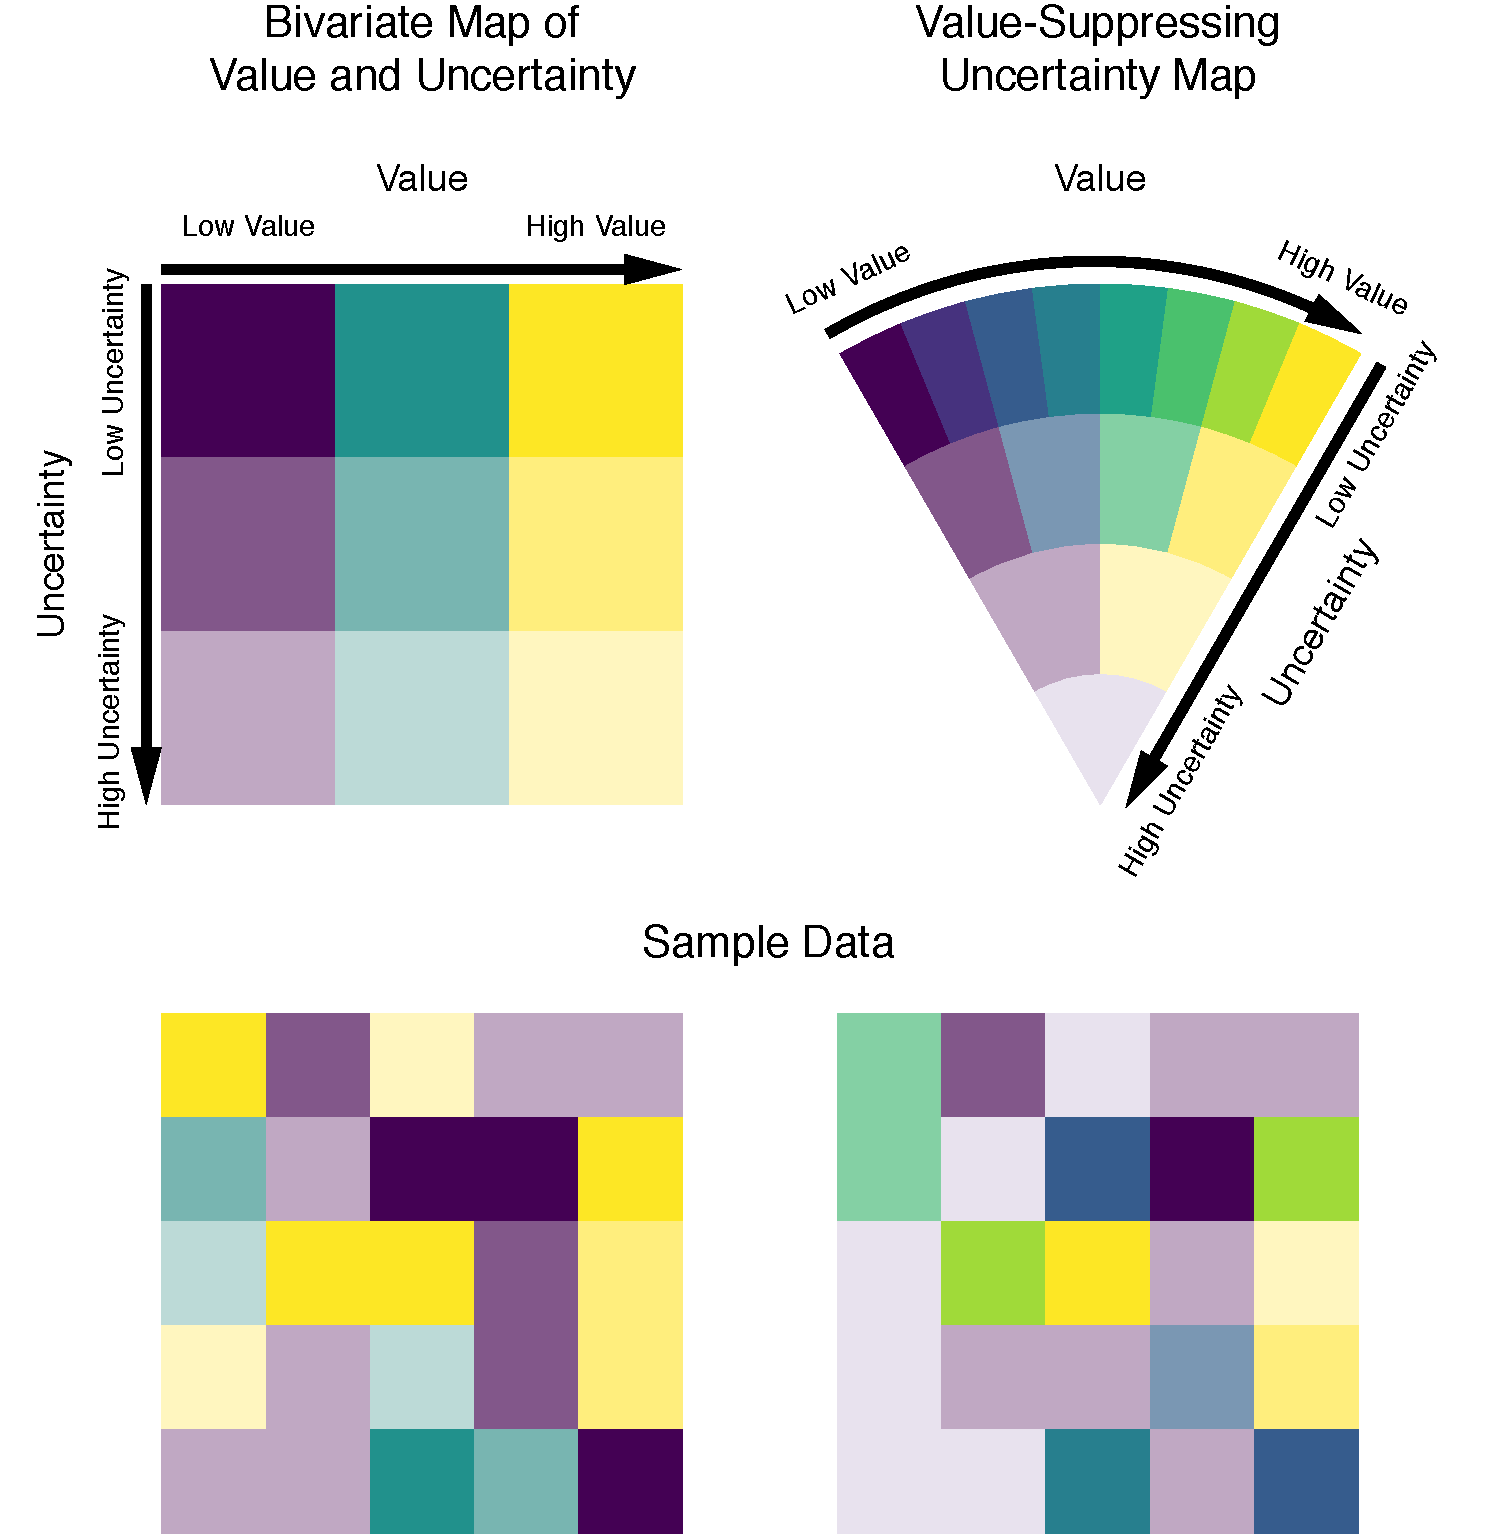
\includegraphics[width=0.9\textwidth]{example.pdf}
		\caption{Lookit! Lookit!}
		\label{fig:teaser}
	}
}

\newcommand{\exampleFig}{
\begin{figure}[t]
	\centering
	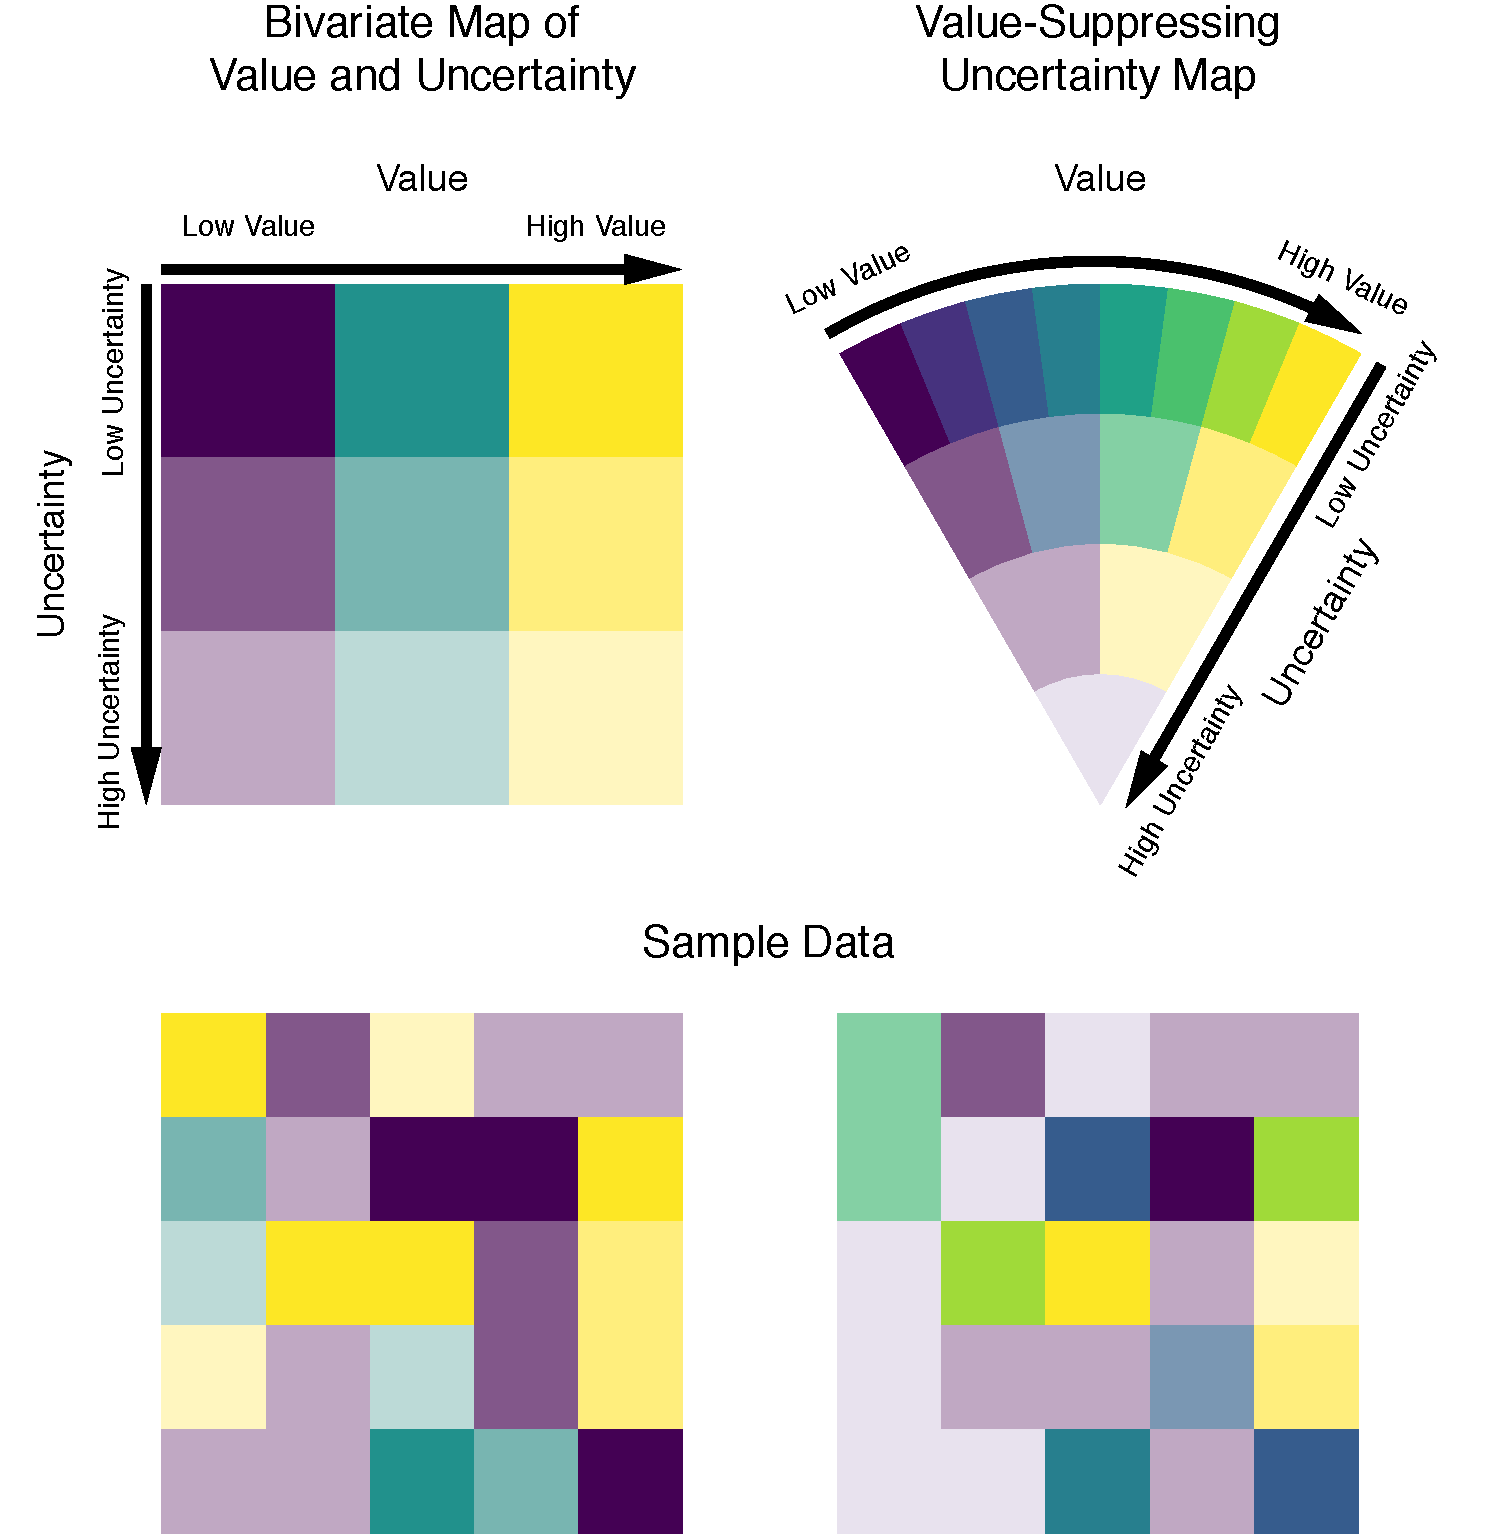
\includegraphics[width=0.9\columnwidth]{example.pdf}
	\caption{A standard bivariate map (left) and a VSUM (right), used to encode an identical 5x5 grid of random data. Both use the same visual channels to encode value (position along the Viridis~\cite{viridis} color map) and uncertainty (lightness and saturation), and have an equal standard of perceptual discriminability (at least 18 units of distance in CIELAB color space between colors). However, highly uncertain values result in colors that are very close together in the bivariate case, meaning the full bivariate map is only 9 bins under these constraints\,---\,a 4x4 map would result in colors that are perceptually too close together. By contrast, the VSUM intentionally reduces bins when uncertainty is high, eventually aliasing all highly uncertain values to the same color. This decision affords more distinct colors in other regions of the map, and so an increase in overall bins to 15. The resulting map suppresses the value of highly uncertain data, but increases the discriminability of data with low uncertainty.}
	\label{fig:example}
\end{figure}
}

\newcommand{\sizeFig}{
	\begin{figure}
		\centering
		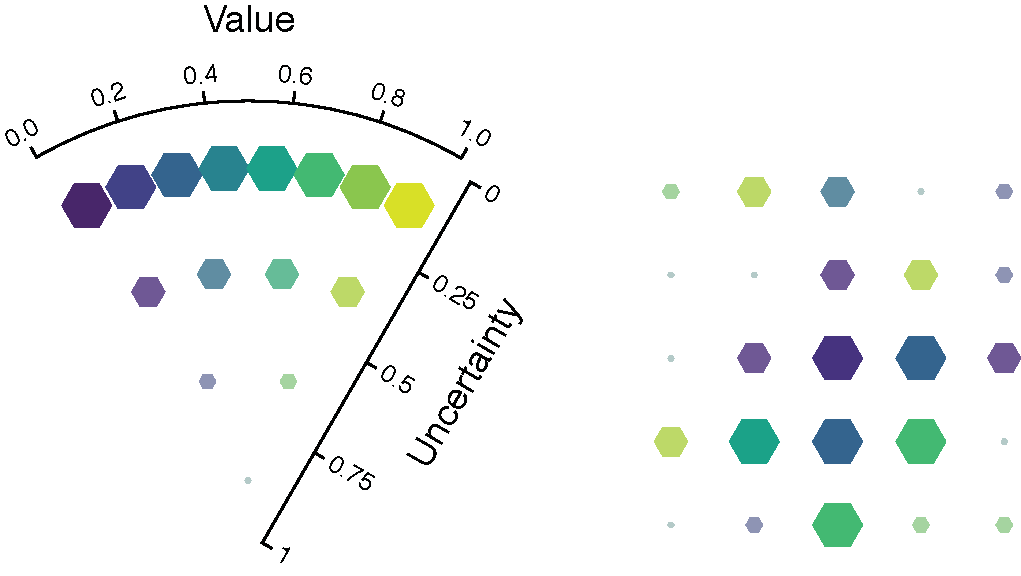
\includegraphics[width=0.9\columnwidth]{size.pdf}
		\caption{A VSUM where value is mapped to color, and uncertainty is mapped to glyph area. As glyphs become smaller, it becomes more difficult to distinguish their colors~\protect\cite{stone2014engineering}. VSUMs, by reducing the number of color categories as uncertainty increases, account for this ambiguity. On the right, the VSUM has been used to encode a 5x5 grid of random data.}
		\label{fig:size}
	\end{figure}
}

\newcommand{\conditionFig}{
	\begin{figure*}[t]
		\centering
		\begin{subfigure}{0.3\textwidth}
			\centering
			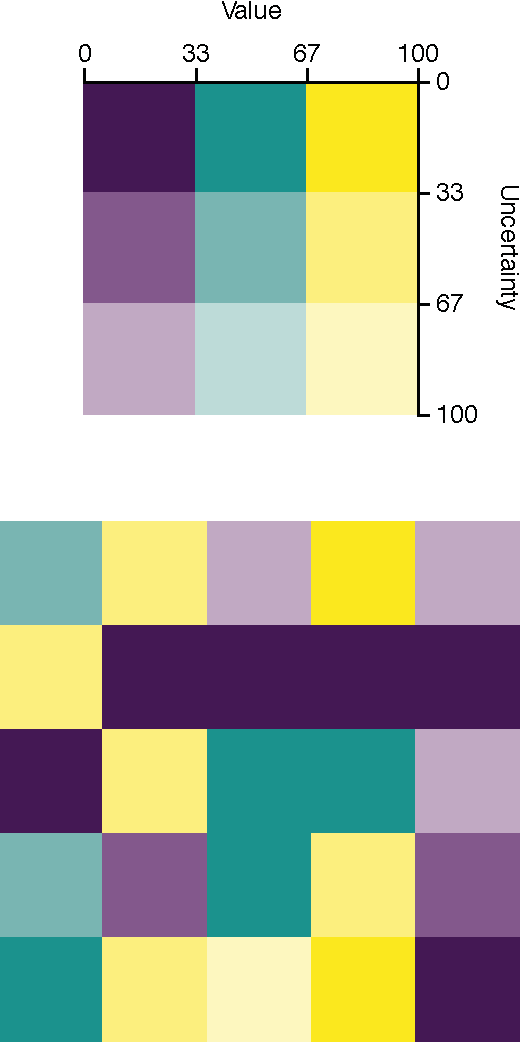
\includegraphics[width=.45\textwidth]{conditions1.pdf}
			\caption{Traditional Bivariate Map}
		\end{subfigure}
		~
		\begin{subfigure}{0.3\textwidth}
			\centering
			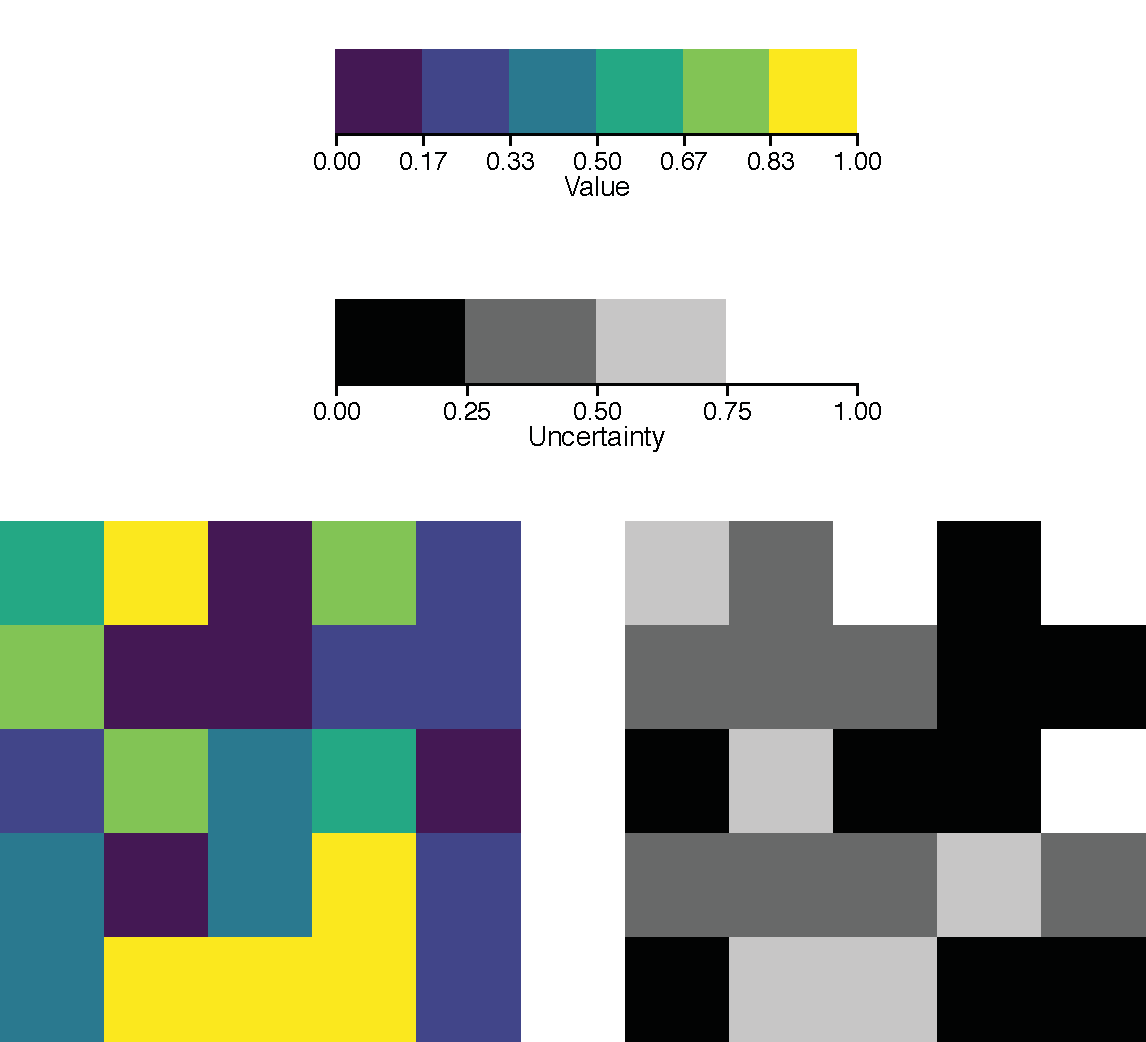
\includegraphics[width=\textwidth]{conditions2.pdf}
			\caption{Juxtaposed Univariate Maps}
		\end{subfigure}
		~
		\begin{subfigure}{0.3\textwidth}
			\centering
			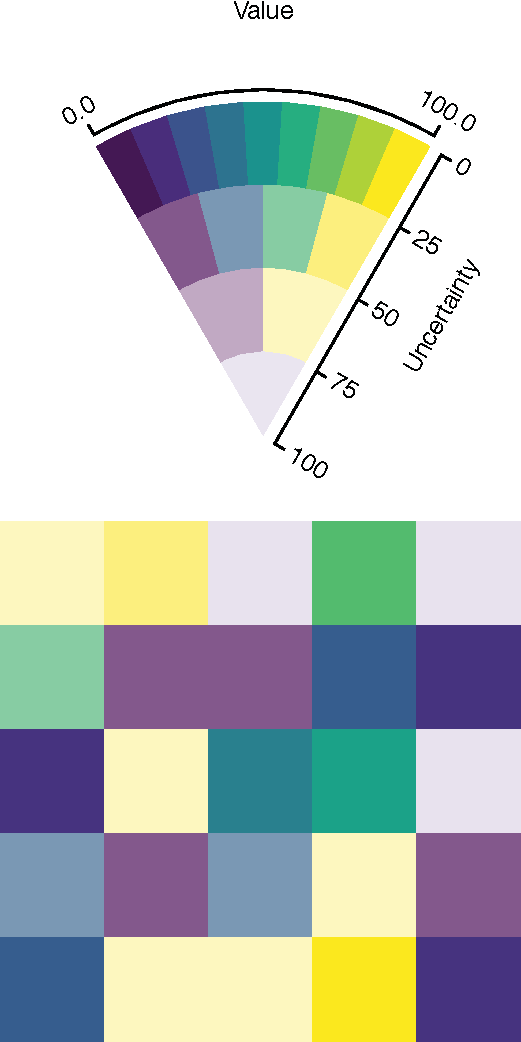
\includegraphics[width=0.45\textwidth]{conditions3.pdf}
			\caption{Value-Suppressing Uncertainty Map}
		\end{subfigure}
		\caption{The three graph types in our evaluation. Bivariate color ramps ensure that there are orthogonal mappings for each combination of value and uncertainty, but, since color channels are not separable, can afford only a few discrete colors before color categories become unacceptably close, perceptually. Juxtaposed maps, by keeping these channels separate, afford a larger range of colors, but require a visual search task to recover both value and uncertainty in a region. VSUMs have many of the advantages of bivariate maps, but assign more color categories to certain data, at the expense of ambiguity when uncertainty is high.}
		\label{fig:conditions}
	\end{figure*}
}

\newcommand{\taskTwoFig}{
	\begin{figure*}
		\centering
		\begin{subfigure}{0.45\textwidth}
			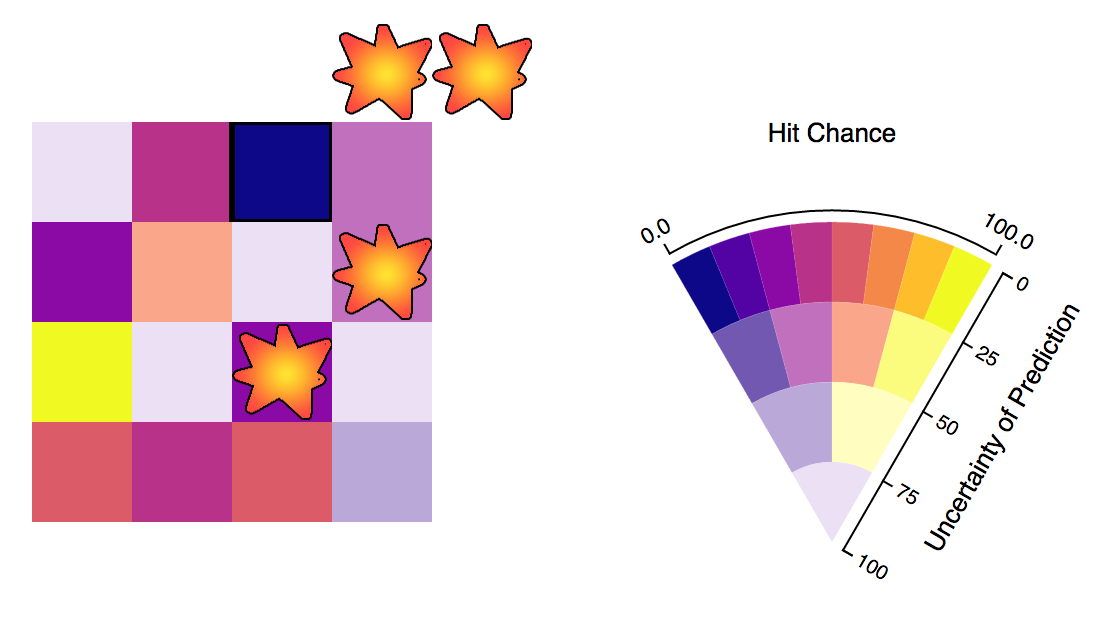
\includegraphics[width=\textwidth]{attack.png}
			\caption{Attacking}
			\label{fig:taskTwoAttack}
		\end{subfigure}
		~
		\begin{subfigure}{0.45\textwidth}
			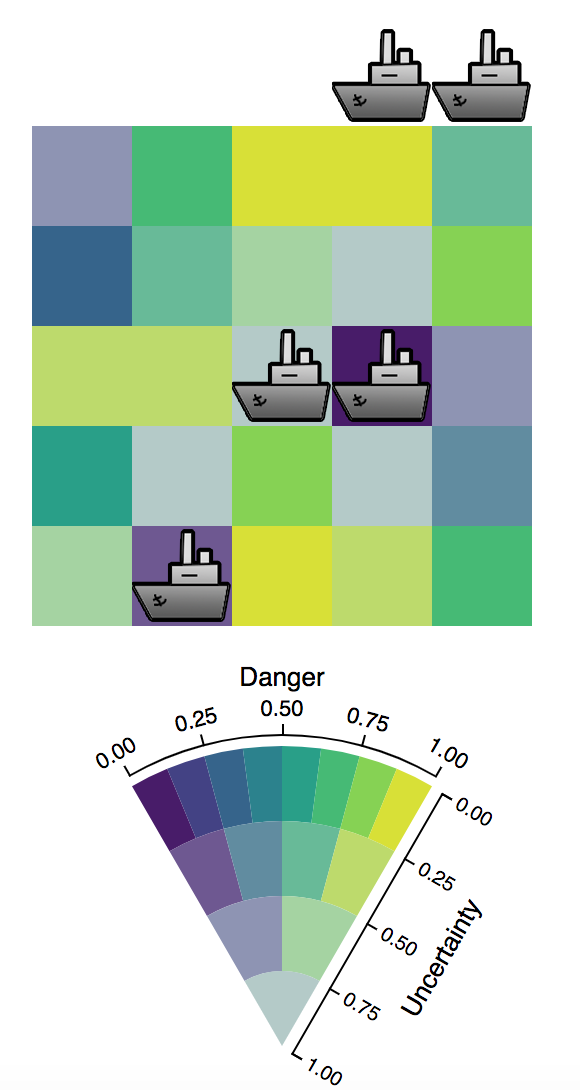
\includegraphics[width=\textwidth]{defend.png}
			\caption{Defending}
			\label{fig:taskTwoDefend}
		\end{subfigure}
		\caption{The two framings of the Prediction task. In the ``attack'' framing, the participant is given a map of predictions of the location of enemy ships, along with the uncertainty in those predictions. The participant should place their missile strikes on locations with a high probability of containing a ship, and with high certainty in this probability. The ``defend'' framing is the opposite task: the participant has a list of likely missile locations, and ought to place their ships on locations with low probability of attack, and high certainty in this probability.}
		\label{fig:taskTwoConditions}
	\end{figure*}
}

\newcommand{\performanceFig}{
	\begin{figure}[t]
		\centering
		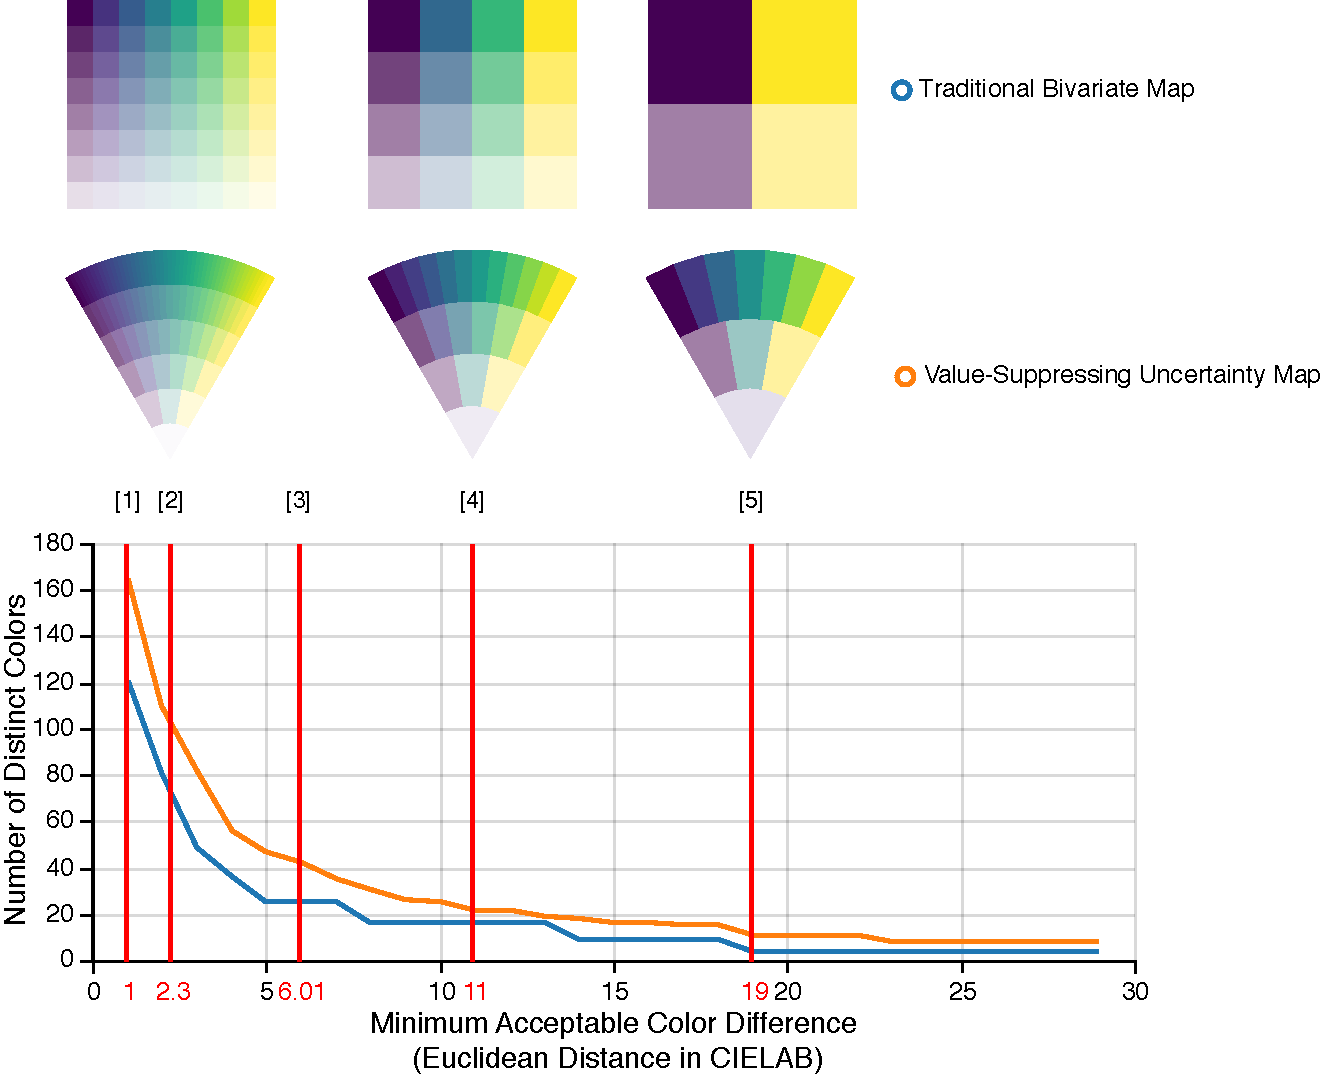
\includegraphics[width=0.9\columnwidth]{performance.pdf}
		\caption{
			The number of discrete color categories in traditional bivariate color maps versus VSUMs, assuming value is encoded by the Viridis color map~\protect\cite{viridis}, and uncertainty is encoded by saturation/value (whiter values are more uncertain). Since these whiter uncertain colors are closer together in CIELAB space, and VSUMs intentionally require fewer color bins in those regions, VSUMs always have more color categories than the corresponding 2D bivariate map. The red lines denote:
		  \textbf{1)} Theoretical 50\% JND from CIELAB specification.
			\textbf{2)} 50\% JND from controlled lab study of Mahy et al.~\protect\cite{mahy1994evaluation}.
			\textbf{3)} 50\% JND from Szafir et al.\protect\cite{szafir2014adapting}.
			\textbf{4)} 50\% JND for small visual targets from Stone et al.~\protect\cite{stone2014engineering}.
			\textbf{5)} The threshold resulting in the simplest possible (2x2) bivariate map.
	    }
		\label{fig:performance}
	\end{figure}
}

\newcommand{\flowFig}{
	\begin{figure}[t]
		\centering
		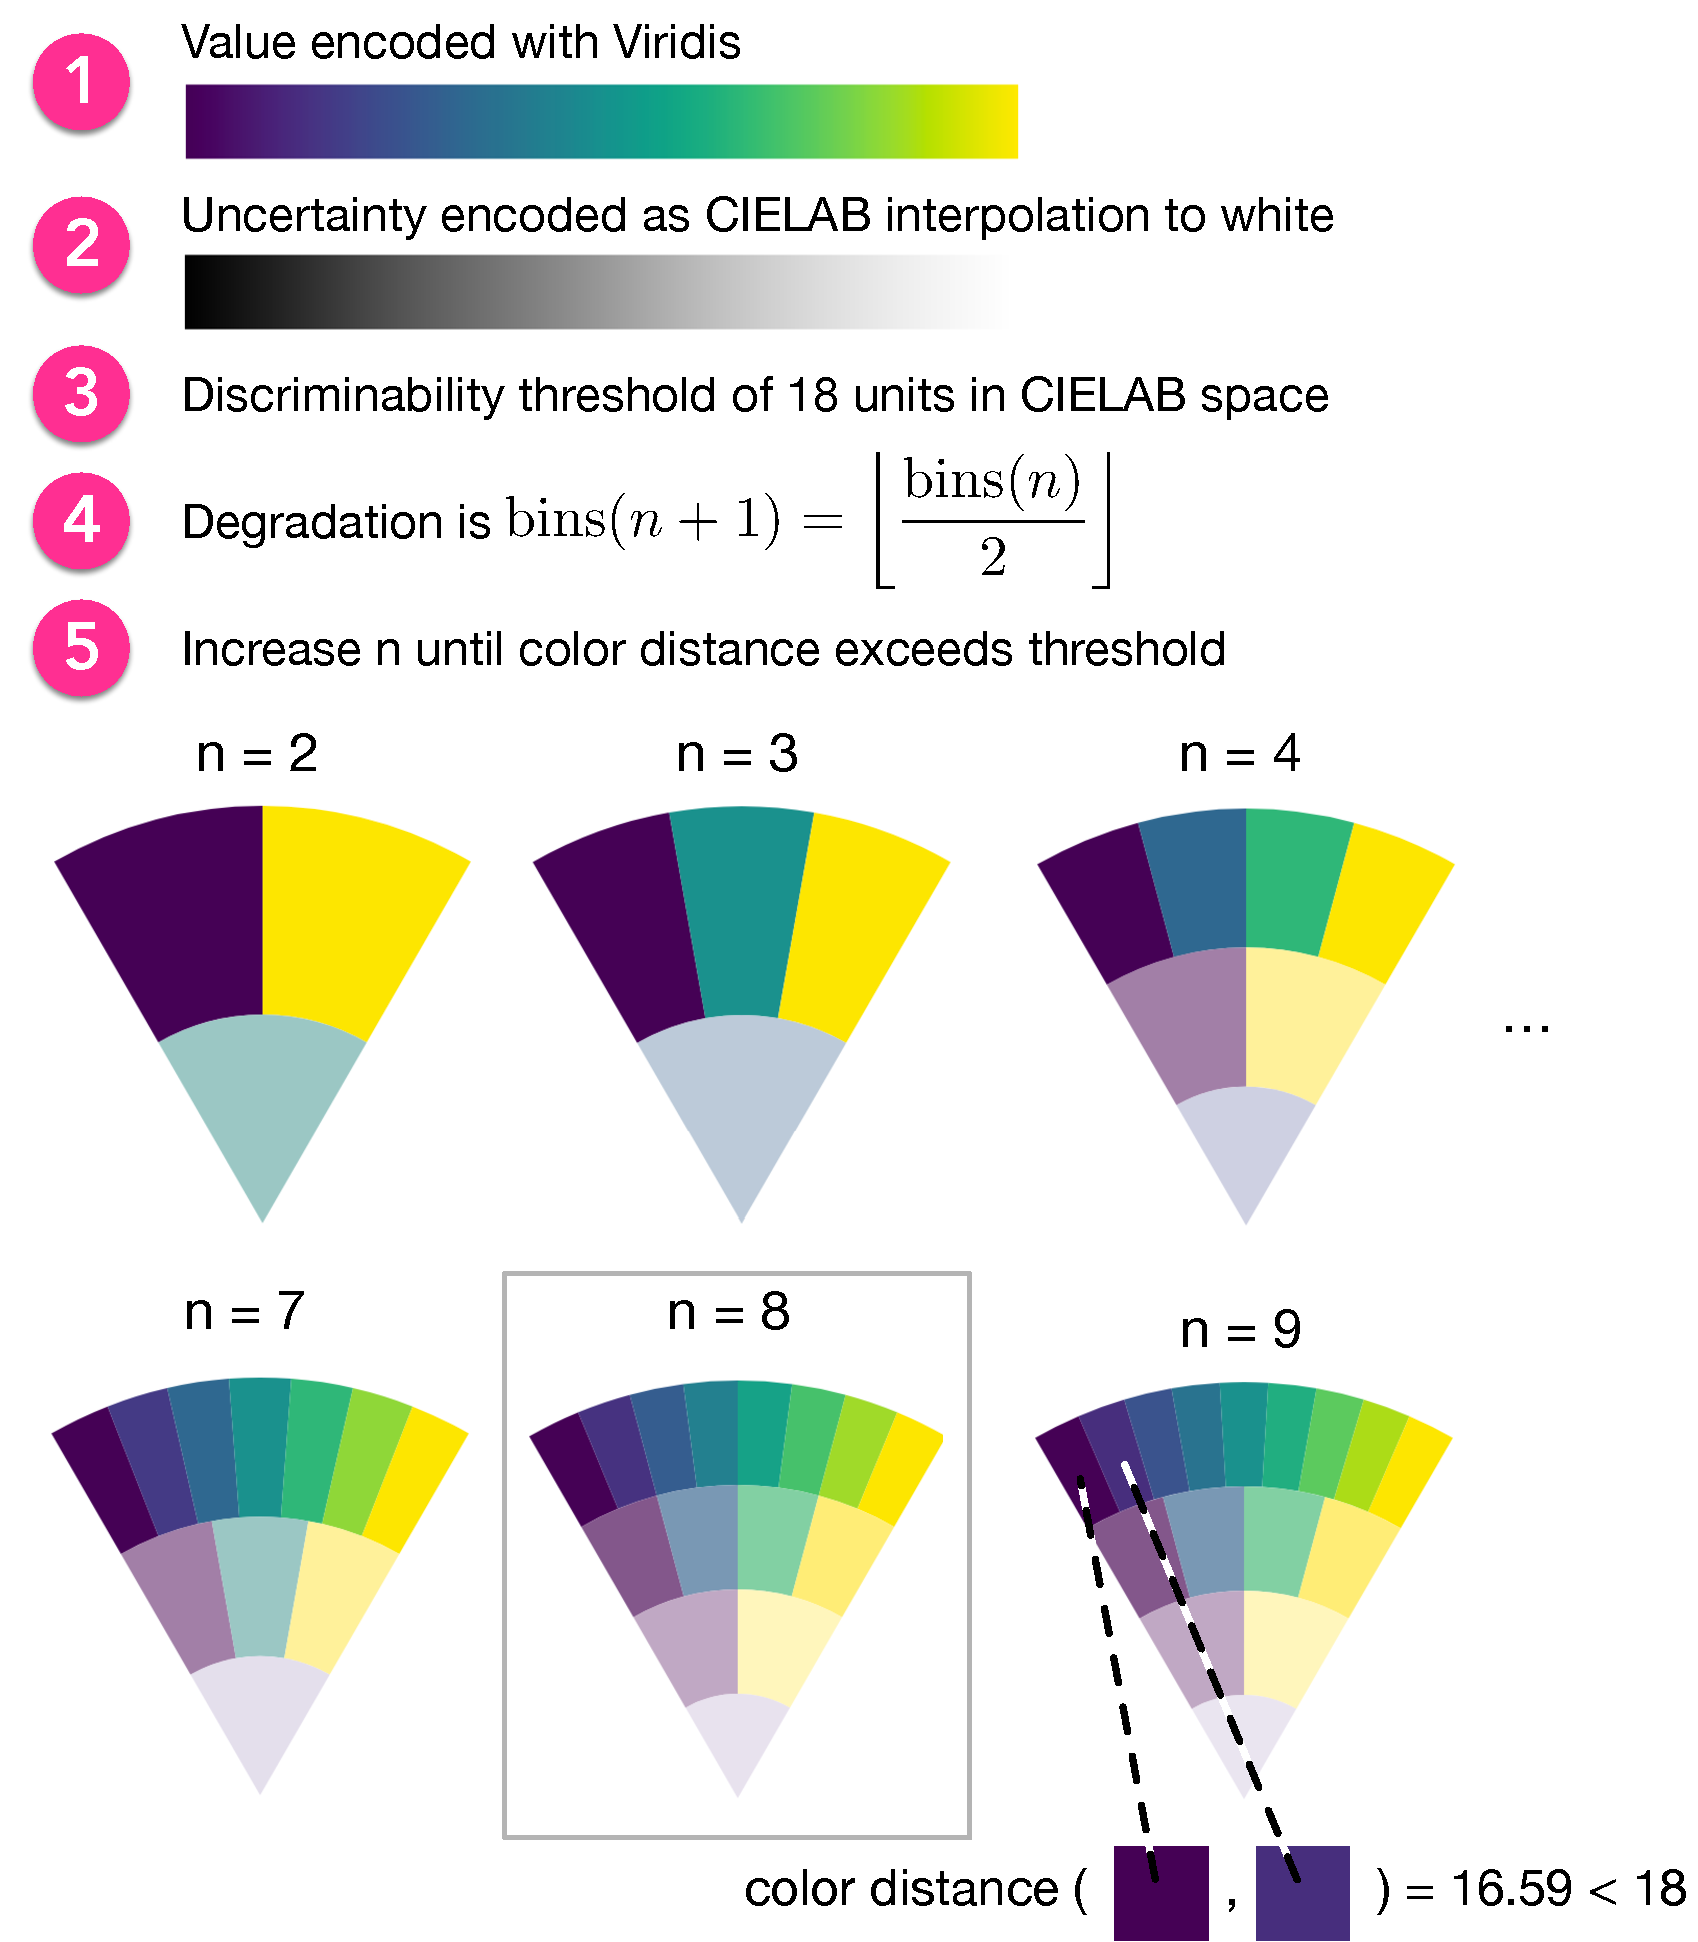
\includegraphics[width=0.95\columnwidth]{flow.pdf}
		\caption{The process for creating a VSUM. VSUMs guarantee that no two marks in the resulting bivariate mapping are perceptually closer than some pre-specified threshold. This guarantee removes some of the issues of non-separability and ambiguity that are otherwise a concern when designing bivariate maps. \\
		In this example two colors from the map for $n=9$ are too close in CIELAB space. Thus, we create a VSUM with $n=8$ color bins at the lowest level of uncertainty.}
		\label{fig:flow}
	\end{figure}
}

\newcommand{\airlineFig}{
\begin{figure}[t]
	\centering
	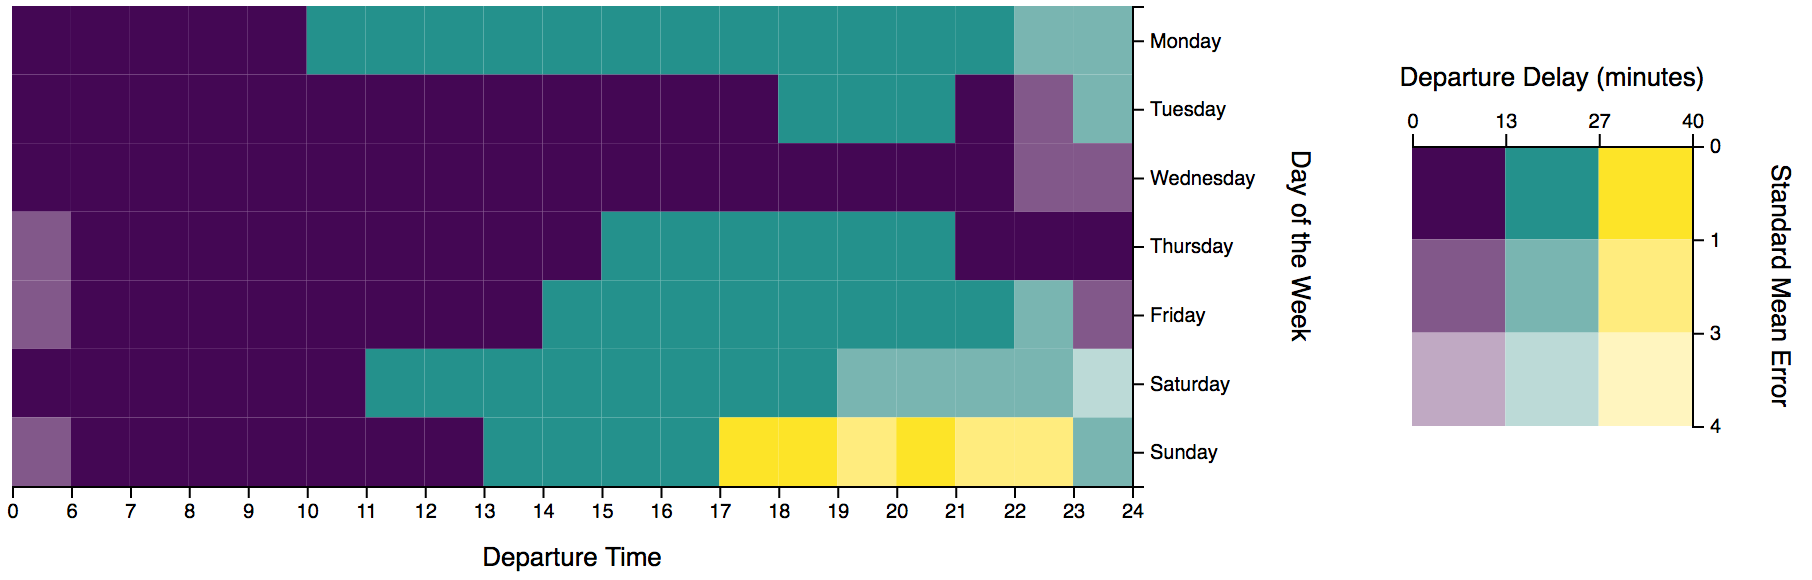
\includegraphics[width=\columnwidth]{airline-2d.png}
	\vspace{-15px}
	\caption{Average departure delay for different times of the day and days of the week visualized with a 2D uncertainty map. Horizontal position is the hour of scheduled departure, and vertical position is the day of the week.}
	\label{fig:airline2d}

	\vspace{10px}

	\centering
	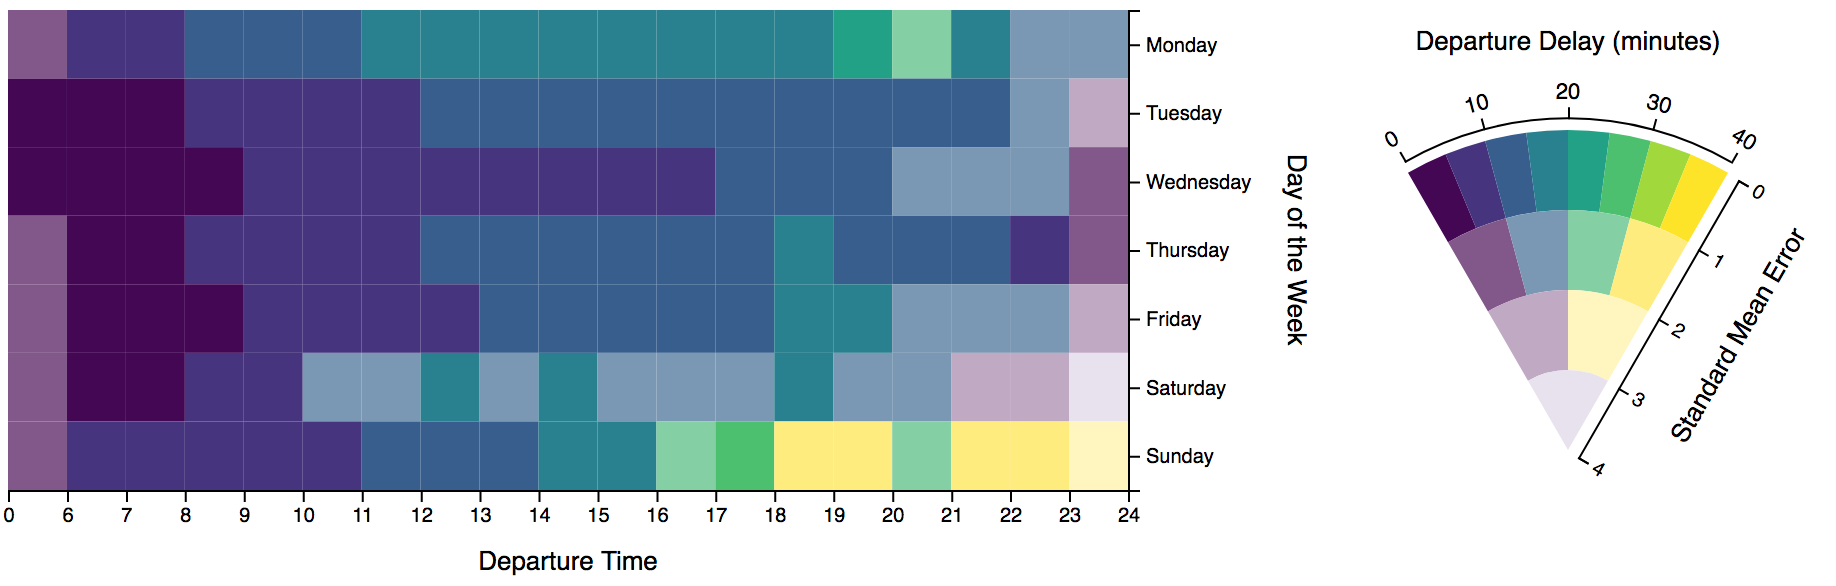
\includegraphics[width=\columnwidth]{airline-vsum.png}
	\vspace{-15px}
	\caption{Flight delay data encoded with a VSUM.}
	\label{fig:airlineVsum}
\end{figure}
}

\newcommand{\viralFig}{
\begin{figure}[t]
	\centering
	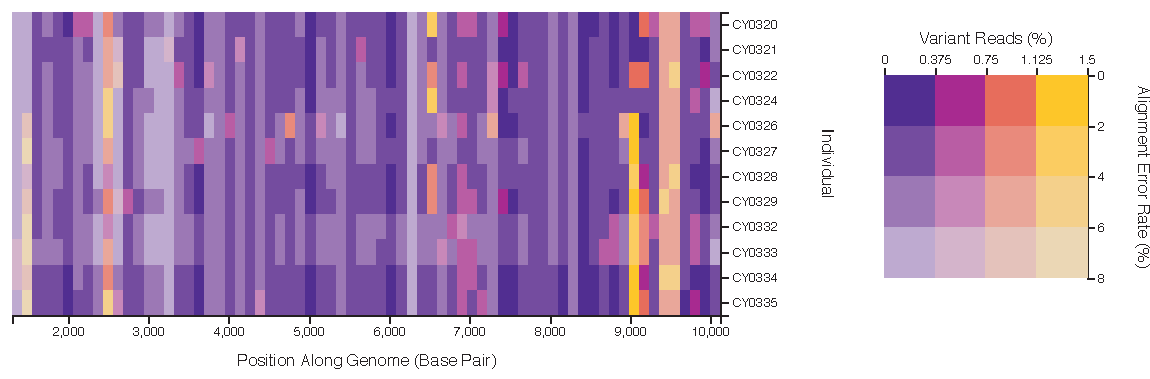
\includegraphics[width=\columnwidth]{viral-2d.pdf}
	\vspace{-15px}
	\caption{Variability for 12 different viral populations of the SIV virus, encoded with a traditional 2D bivariate map. Horizontal position denotes location along the SIV genome. Each row is the viral population of a different infected animal. Error in aligning short reads can lead to poor quality data, and so the amount of these errors is encoded as the uncertainty. }
	\label{fig:viral2d}

	\vspace{10px}

	\centering
	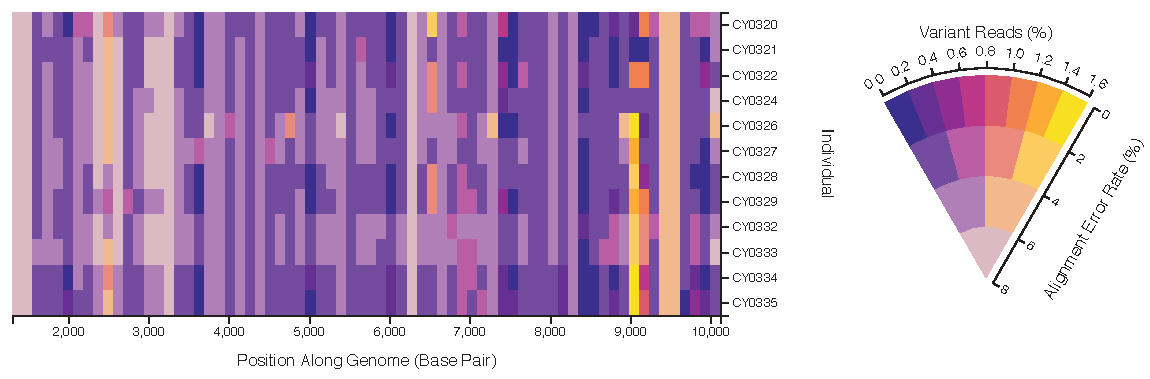
\includegraphics[width=\columnwidth]{viral-vsum.pdf}
	\vspace{-15px}
	\caption{Variability for 25 different viral populations of SIV, encoded with a VSUM. The magnitude of mutation rate, as well as the generally poorer quality of data towards the end of the sequence, is more readily visible than with the traditional bivariate color map. }
	\label{fig:viralVsum}
\end{figure}
}

\newcommand{\responseTimeFig}{
	\begin{figure}[t]
		\centering
		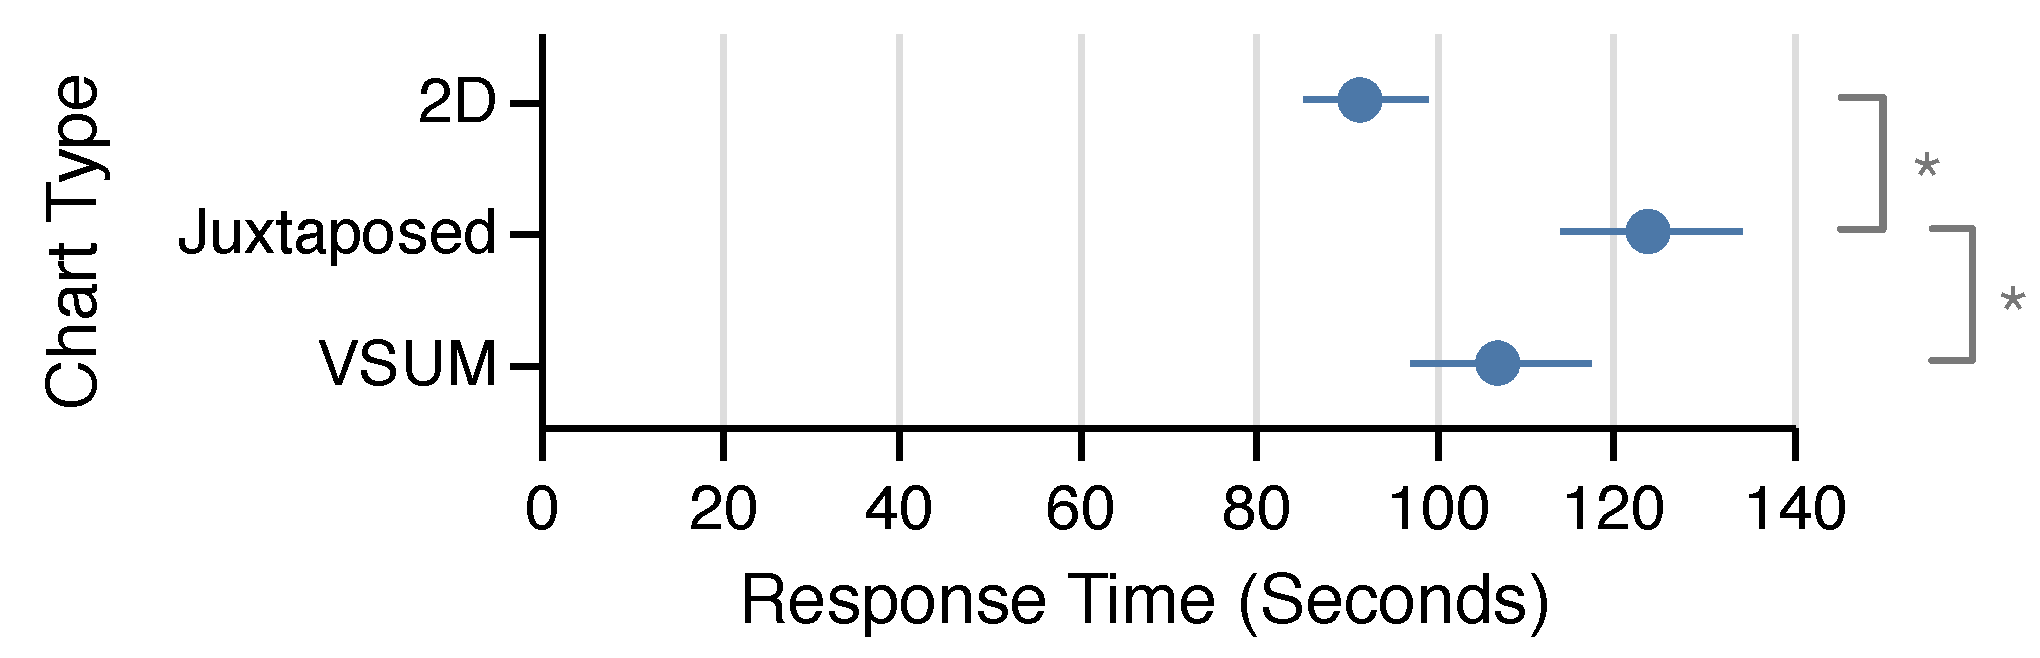
\includegraphics[height=2.4cm]{rt1.pdf}
		\caption{The effect of chart type on response time for the identification task. Juxtaposed maps of value and uncertainty introduce a visual search task, increasing the time to complete even simple tasks involving both value and uncertainty information. The confidence intervals are bootstrapped 95\% CIs of trimmed means.}
		\label{fig:rt1}
	\end{figure}
}

\newcommand{\accuracyFig}{
	\begin{figure}[t]
		\centering
		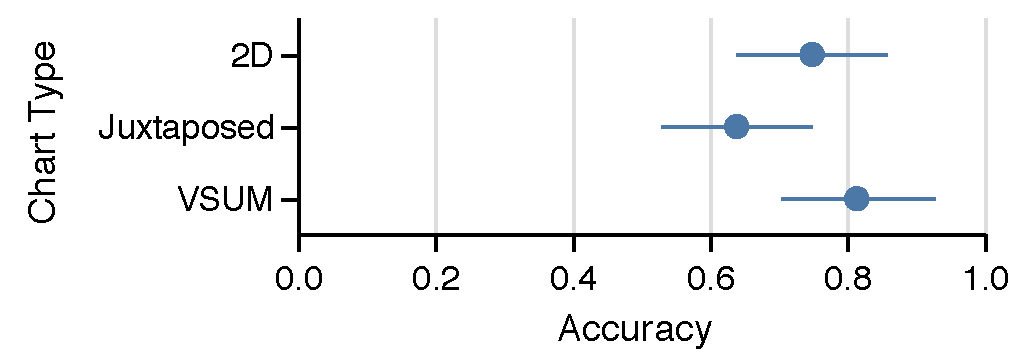
\includegraphics[height=2.4cm]{accuracy1.pdf}
		\caption{The effect of chart type on accuracy for the identification task. VSUMS are similarly accurate for simple search tasks as more traditional bivariate visualizations, despite containing additional colors categories, and having a more complex relationship between uncertainty, value, and color than traditional charts. The confidence intervals are bootstrapped 95\% CIs of trimmed means.}
		\label{fig:accuracy1}
	\end{figure}
}

\newcommand{\uncertaintyFig}{
	\begin{figure}[t]
		\centering
		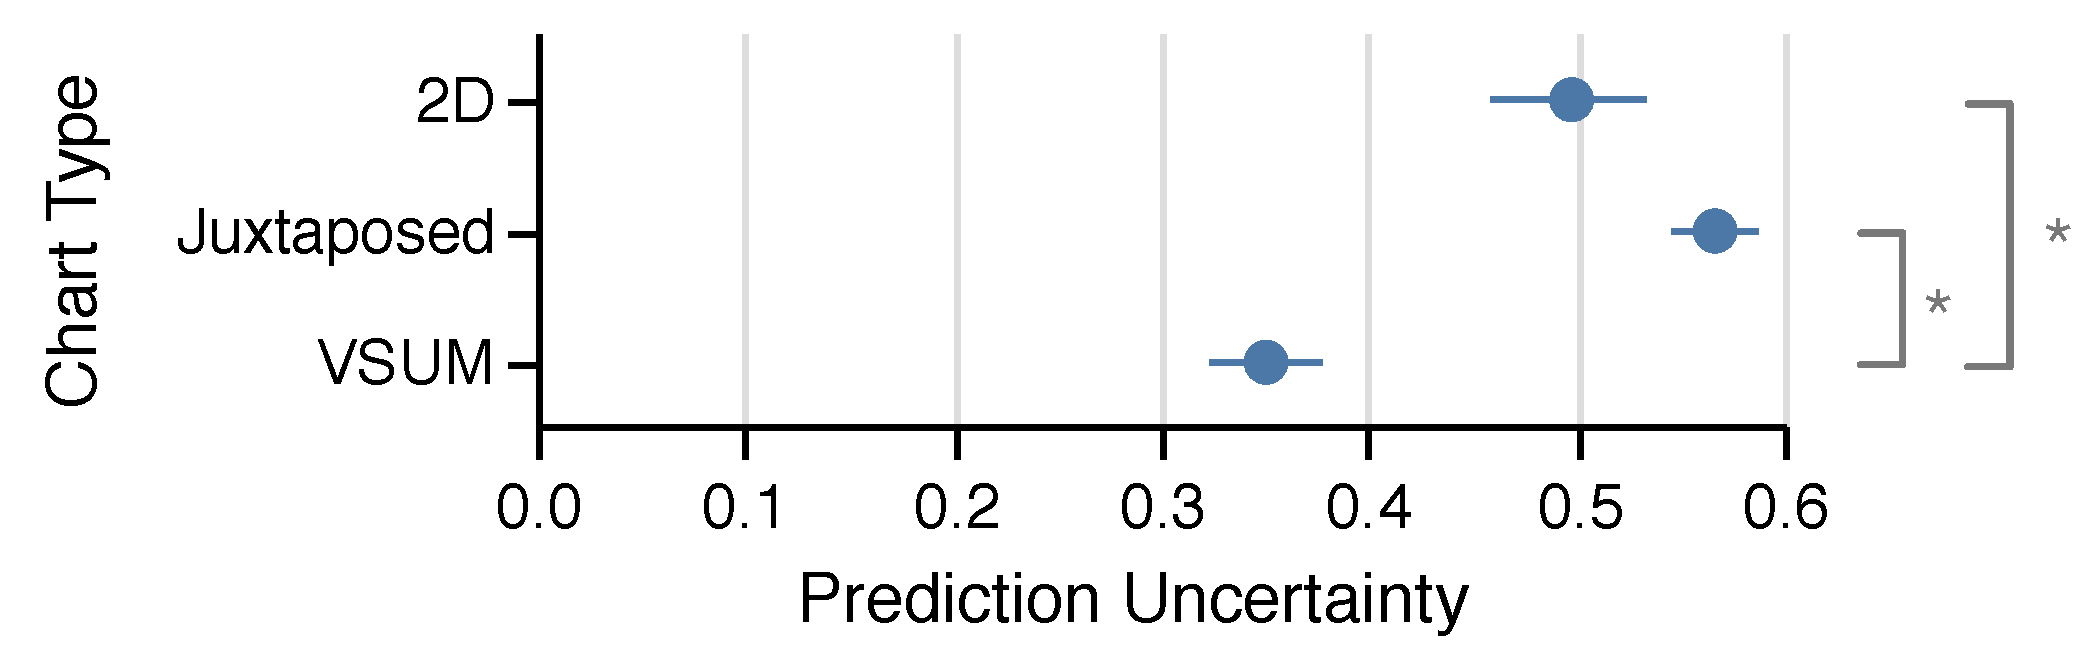
\includegraphics[height=2.4cm]{uncertainty2.pdf}
		\caption{The effect of chart type on the average uncertainty in predictions for the prediction task. By reducing the number of color categories as uncertainty increases, VSUMs encourage more caution in predictions, making people less likely to consider data with strong, but spurious patterns. The confidence intervals are bootstrapped 95\% CIs of trimmed means.}
		\label{fig:uncertainty2}
	\end{figure}
}

\newcommand{\strategyFig}{
	\begin{figure}[t]
		\centering
		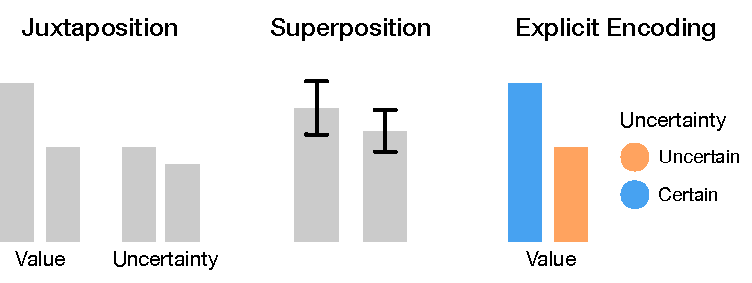
\includegraphics[width=.9\columnwidth]{strategies.pdf}
		\caption{Strategies for encoding uncertainty information along with values. From left to right: encode uncertainty is a separate visualization, overlay uncertainty information, or encode uncertainty with a separate channel.}
		\label{fig:strategies}
	\end{figure}
}

%\teaserFig
%% A teaser figure can be included as follows, but is not recommended since
%% the space is now taken up by a full width abstract.
%\teaser{
%  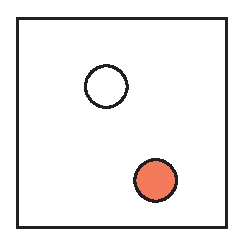
\includegraphics[width=1.5in]{sample.eps}
%  \caption{Lookit! Lookit!}
%}

%% Abstract section.
\abstract{
	
	% uncertainty-aware decisions.
	% refrain from making a decision
	% integrate uncertainty with the display
	% value-suppressing encodings
	% provide greater visual discriminability for values with high certainty, but alias together uncertain values
	% ran a study
	% results indicate X
	
Uncertainty is a vital concern in many datasets. Visualizations often use bivariate mappings to encode value and uncertainty simultaneously. Due to interference between visual channels, these bivariate maps are limited in discriminability. We contribute Value-Suppressing Uncertainty Maps (VSUMs), an encoding technique that intentionally impairs value discrimination as uncertainty increases. In contrast to traditional bivariate maps, VSUMs alias values when uncertainty is high: expected values with lower uncertainty can be more precisely compared, whereas similar values with higher uncertainty are made harder to differentiate. By making informed binning decisions, VSUMs seek to better use the limited budget of discriminable marks in bivariate maps, and dissuade analysts from making decisions based on data with high uncertainty. We demonstrate several examples of VSUMs and present a crowdsourced evaluation showing that, compared to traditional bivariate maps, VSUMs bias analysts to more heavily weight uncertainty information in decision-making tasks.
	
} % end of abstract

%% ACM Computing Classification System (CCS). 
%% See <http://www.acm.org/class/1998/> for details.
%% The ``\CCScat'' command takes four arguments.

\keywords{Uncertainty Visualization, Color Perception, Thematic Maps, Semiotics.}

%\CCScatlist{ 
%  \CCScat{K.6.1}{Management of Computing and Information Systems}%
%{Project and People Management}{Life Cycle};
%  \CCScat{K.7.m}{The Computing Profession}{Miscellaneous}{Ethics}
%}

%% Copyright space is enabled by default as required by guidelines.
%% It is disabled by the 'review' option or via the following command:
% \nocopyrightspace

%%%%%%%%%%%%%%%%%%%%%%%%%%%%%%%%%%%%%%%%%%%%%%%%%%%%%%%%%%%%%%%%
%%%%%%%%%%%%%%%%%%%%%% START OF THE PAPER %%%%%%%%%%%%%%%%%%%%%%
%%%%%%%%%%%%%%%%%%%%%%%%%%%%%%%%%%%%%%%%%%%%%%%%%%%%%%%%%%%%%%%%%

\begin{document}

%% The ``\maketitle'' command must be the first command after the
%% ``\begin{document}'' command. It prepares and prints the title block.

%% the only exception to this rule is the \firstsection command
\firstsection{Introduction}

\maketitle

%% \section{Introduction} %for journal use above \firstsection{..} instead


% What this section needs to do:
% Uncertainty is important!
% What do we mean by ``well-integrated'' uncertainty?
% Scope down to thematic maps
% Juxtapose/superimpost distinction?
% Position bivariate maps (tacitly or explicitly) as state of the art
% Teaser image showing what we mean

Uncertainty is an inescapable component of collecting, presenting, and using data. A common goal in the communication of uncertainty is promoting \textbf{uncertainty-aware decisions}--- that is, the audience should be aware of the risks and rewards of certain decisions, modulate their confidence in their conclusions, and perhaps refrain from making a decision at all if there is too much uncertainty.  A way that designers can contribute to this goal is by ensuring that uncertainty information is \textbf{well-integrated} with the rest of the data. That is, it should be difficult to discount or ignore the uncertainty in a dataset. Simultaneous presentation of uncertainty and value necessitates the construction of a bivariate map--- a relation, in terms of visual variables, between 2-tuples $(\text{value}, \text{uncertainty})$ and mark properties. The design of bivariate maps is difficult and, due to the interference and interplay between different visual variables, often leads to maps with few discriminable categories. 

In this paper, we present \textbf{Value-Suppressing Uncertainty Maps} (VSUMs) for integrating data and uncertainty information in thematic maps. VSUMs intentionally alias together data values with high uncertainty, affording greater discriminability as certainty increases. Rather than a traditional two-dimensional bivariate map, with differing outputs for each combination of value and uncertainty, VSUMs can be thought of as arcs: as uncertainty increases, values are mapped to smaller and smaller sets of outputs, culminating in a singularity where all inputs are mapped to an identical, highly uncertain mark regardless of their data value. Figure \ref{fig:example} shows an example of a VSUM, compared to a more traditional bivariate map. In this work, we describe the motivations behind the use of VSUMs, examples of their utility for decision-making under uncertainty, and assess VSUMs in a crowd-sourced experiment. Our experimental results indicate that VSUMs promote better integration between uncertainty and data: X.

\exampleFig 
\section{Related Works}

% What this section needs to do:
% State of the art in uncertainty vis, with heavy emphasis on MacEachren & co. 
% Bivariate maps are hard!
% Binning colormaps is de rigueur
% The variables we'd want to use for uncertainty (like value or alpha or size) mess with color discriminability

Despite the acknowledged importance of uncertainty in understanding data, explicit representation of uncertainty often missing from visualizations~\cite{boukhelifa2009uncertainty}. This is partially due to the complexity of uncertainty as a concept. In typologies from Thomson et al~\cite{thomson2005typology} and Buttenfield \& Beard~\cite{buttenfield1994graphical}, the authors note that many, occasionally contradictory, concepts can fall under the category of ``uncertainty,'' including data quality, sampling error, credibility, and provenance. This complicates 
 
In their reviews of the state of the art in uncertainty visualization in the field, Greithe et al.~\cite{griethe2006visualization} and Brodlie et al.~\cite{brodlie2012review} present lists of potential techniques for conveying uncertainty in concert with data. Some of these options (interaction, animation, and sonification) are not applicable for static charts; even for dynamic charts, many users do not interact with charts in sufficient detail to recover uncertainty information~\cite{nyt2016}. While we acknowledge the potential utility of these techniques in uncertainty visualization (for instance, the animation used to convey sampling error in Hullman et al.'s \emph{HOPs}~\cite{hullman2015hypothetical}), we limit the scope of our discussion to techniques which center on static charts.

To support our goal of making uncertainty information well-integrated with data, we focus on the techniques of \textbf{juxtaposition} (where uncertainty is presented alongside the data), \textbf{superposition} (where additional glyphs are overlaid on top of the data), or \textbf{explicit encoding} (where a spare visual channel, such as color, is used to encode the uncertainty simultaneously with the data). Gleicher et al.~\cite{gleicher2011visual} explore these three strategies from the perspective of affording \textbf{comparisons}; here, we examine them from the perspective of \textbf{information fusion}.

Juxtaposition creates two explicit visualizations: an ``uncertainty map'' and a ``data map.'' MacEachren~\cite{maceachren1992visualizing} portrays uncertainty visualization as the design problem of how to \emph{unify} these two maps, and so this explicit separation can be counterproductive to the goal of information fusion. Juxtaposition also creates an additional search task for viewers, who must register hot spots in one map with corresponding features of the other map. Nevertheless, especially in cases where the quantification of uncertainty is a separate analysis process from the measuring of data values, juxtaposition is a common design tactic for conveying uncertainty.

Superposition, or the overlay of glyphs representing uncertainty on top of a data map, is another common strategy.  Ware's~\cite{ware2009quantitative} \emph{textons} are an example of this strategy: monochrome glyphs that can encode an ordinal variable, or a binned quantitative variable. Greithe et al.~\cite{griethe2006visualization} and MacEachren~\cite{maceachren1992visualizing,maceachren1998visualizing} present other examples of this technique, including overlaid grids with ``fuzzy'' lines to indicate uncertainty, or overlaid treemaps with coarser and coarser resolution in uncertain regions. Costs to this approach include obscuring the underlying datamap (which can cause uncertainty information to dominate the display~\cite{brodlie2012review}), potential visual interactions (for instance, simultaneous contrast effects) that can impair the legibility of glyphs, and the necessity of performing spatial binning in order to ensure that there are a discrete number of uncertainty glyphs. How this binning is performed can introduce undesirable artifacts on the resulting visualization, and suppress important signals, or highlight spurious ones \cite{battersby2016shapes}. 

VSUMs are intended for situations where designers explicitly encode uncertainty simultaneously with data. In addition to overcoming the drawbacks of the other techniques mentioned in this section, we believe that explicit encoding represents the most general form of the solution of how to fuse uncertainty information with data. The most pressing design decisions for explicit encoding are 1) which visual variable to use to encode uncertainty and 2) how to design bivariate maps which afford the encoding of both value and uncertainty. We deal with these two questions in greater detail below.

\subsection{Visual Variables for Representing Uncertainty}

The decision to explicitly encode uncertainty increases the dimensionality of the data, and so requires the use of (at least one) additional visual channel ~\cite{brodlie2012review}. Uncertainty therefore inherently increases the visual complexity of a visualization. When the data are already complex to convey, and many of the more common or accurate visual variables are in use, allocating an additional dimension is non-trivial. As the number of dimensions increases, finding visual variables that are both perceptually accurate (in either estimation of quantity or discrimination of category) as well as perceptually separable from all the other encoding channels, becomes more and more difficult.

A further hurdle is that not all visual variables are well-suited for conveying uncertainty. MacEachren et al.~\cite{maceachren2012visual} evaluate a number of visual variables with respect to their \emph{semiotic fit} for representing uncertainty. They observe that certain visual variables such as blurriness and transparency seem to have a more intuitive connection to uncertainty than other variables such as shape or hue. Unfortunately, Boukhelifa et al.~\cite{boukhelifa2012evaluating} discover that many visual variables habitually used for conveying uncertainty, such as blur and value, are also difficult to estimate. This results in a preference/performance gap where designers must choose between encoding uncertainty in a way that is intuitive but error prone, or use higher fidelity channels that are difficult to interpret. 
 
\subsection{Bivariate Maps}

In for visualizations like choropleth maps, heatmaps, or treemaps, visual channels such as position and length are reserved for data variables other than value (such as geographic location or relative size). In these situations, data value is habitually encoded using color. Colors in such univariate quantitative color maps should be sufficiently far apart as to be perceptually distinguishable~\cite{ware1988color}, and vary in lightness as well as hue in order to afford an implicit ordering of value~\cite{borland2007rainbow,rogowitz2001blair}. Given these constraints, and the perceptual non-orthogonality of color channels, the construction of \emph{bivariate} color maps is difficult. Bivariate color maps out to be separable (the two variables can be distinguished independently) but also expressive and easy to interpret. Bivariate maps with these constraints are often limited to relatively few categories (say, a 3x3 matrix as in Figure \ref{fig:example}) \cite{robertson1986generation,trumbo1981theory}. Even so, the resulting bivariate maps are often difficult to interpret \cite{wainer1980empirical}.


Dunn~\cite{dunn1989dynamic} attempts to circumvent these issues by dynamically allocating bins to the bivariate map. Since distinct, separable colors are limited, the dynamic approach allocates bins to regions of the highest utility. For instance, placing the dividing line between bins in areas aligned with a trend line allows the color to encode information about the sign of the residual with respect to each variable. This insight, that the bins in a bivariate map are a limited resource and so should be ``spent'' wisely, drives the creation of VSUMs, which allocate more bins in a bivariate map to regions with higher certainty. 


\section{Value-Suppressing Uncertainty Maps}

We present Value-Suppressing Uncertainty Maps, a technique for creating bivariate maps of data \emph{value} and \emph{uncertainty}. These maps circumvent the issues in the creation of traditional bivariate maps by making the following assumptions:

\begin{enumerate}
	\item \textbf{Designers have a limited budget of discriminable marks.} That is, viewers cannot easily or reliably discriminate between an infinite number of categories. Rather than accept this perceptual ambiguity, designers ought to \emph{alias} together marks into a finite, but sufficiently discriminable, set.
	\item \textbf{Uncertain values should have less weight than certain values.} Weight, in this case, might mean literal visual weight, or impact on the decision-making process. 
\end{enumerate}

%MC this paragraph is a little iffy, and sort of "the lady doth protest too much" territory. we might be able to get away with "people bin colors all the time. and in fact, you really should be binning your colors anyway."
The first assumption seems to contradict the \emph{expressiveness principle}~\cite{mackinlay1986automating}, where the visual encoding of the data should reflect the composition of the data. For instance, if my data are a collection of measurements of some continuous variable, then it would make sense to encode these data using a continuous \emph{visual} variable, which would then mean an arbitrary number of potential marks. For instance, a bar can have an arbitrary, non-integer heights. However, for many visualizations, the perceptual ambiguity caused by having marks that cannot be reliably disambiguated is higher than the gain from having a visual encoding that maps readily to the backing data. Padilla et al.~\cite{padilla2017evaluating} present one such example, where binned heatmaps results in higher accuracy in tasks than in continuous heatmaps.

In some cases, this second assumption is violated. For instance, an analyst might be interested in ``long tail risks'' or other ``black swan events,'' where the impact of an value, no matter how uncertain, must be considered and planned for~\cite{taleb2011black}. Other analysis tasks (such as filtering out outliers), require increased, rather than decreased, discrimbinability when uncertainty low. However, for many information fusion tasks, the assumption is that uncertainty is related to data quality, or the certainty of particular data values \cite{riveiro2007evaluation}. As with null hypothesis significance testing, the aim would then be to avoid Type I errors, where patterns arising from statistical noise or measurement error are interpreted as significant signals.

If both of these assumptions hold, then it follows that the designer of a bivariate map should allocate more mark types to certain values, and fewer mark types to uncertain values. VSUMs codify this decision by \emph{reducing the number of mark categories for representing value as uncertainty increases.} The general VSUM algorithm is as follows:

\begin{enumerate}
	\item \textbf{Select a visual variable to encode value}. In most cases in this paper, this variable is position along some established color scale.
	\item \textbf{Select a visual variable to encode uncertainty}. We choose variables that have a somewhat high semiotic connection with uncertainty (such as lightness and size), but still have a reasonable number of perceptually discriminable layers (as opposed to other, more intuitive channels such as blur or sketchiness).
	\item \textbf{Select a discriminability threshold}. This is some minimum distance, in perceptual space, between marks. For many visual variables (such as length or hue), the perceptual discriminability between marks has been assessed in prior literature, and so the only step is to choose some value in terms of the just noticeable distance (JND). For less common visual variables, this perceptual space must be built up empirically (as in Demiralp et al.~\cite{demiralp2014learning}).
	\item \textbf{Choose how quickly categories \emph{degrade}}. That is, if there are $n$ bins at some uncertainty level $m$, how many bins should there be when uncertainty increases to level $m+1$? In Figure \ref{fig:example}, this function is $\left \lfloor {\frac{n}{2}}\right \rfloor$, meaning that the number of value bins decreases by half for each level of uncertainty bins. If there is too much degradation, then there are fewer levels of uncertainty. If there is no degradation, the resulting map is just a traditional bivariate map. 
	\item \textbf{Choose the largest number of initial categories $n$ such that the discriminability threshold is met.} For each pair of marks in the map, perform a pairwise comparison of discriminability. If no marks are perceptually ambiguous by the standards of your threshold, then the map is complete. Otherwise, decrement $n$. 
\end{enumerate}

Figure X shows this process in detail, and how it can be used to generate a bivariate map for presenting uncertainty. Javascript code for generating VSUMs given arbitrary d3 quantitative scale functions is available at \url{URL REMOVED FOR REVIEW}.

Correll et al. use a version of VSUMs in their LayerCake genomics visualization tool \cite{correll2015layercake,correll2011visualizing}, where marks representing genomic data with insufficient certainty are mapped to a smaller and smaller set of increasingly grey colors, creating the effect of uncertain values retreating into ``fog'' while highly certain values remain prominent. Other bivariate visualizations implicitly alias together uncertain values. For instance, if uncertainty is encoded by transparency, a maximally uncertain glyph may be entirely transparent, and so impossible to distinguish from any other maximally uncertain glyph. Other channels with a semiotic connection ot uncertainty, such as saturation, value, blur, or size, also have deleterious effects on the disambiguation of colors and shapes. In both of these cases, this property of aliasing is ad hoc, and places no guarantees on the discriminability of colors. The binning and degradation approach of VSUMs makes this choice to alias values explicit to both the designer and the viewer, and results in a bivariate mapping with known perceptual properties.

\subsection{Design Considerations}

\performanceFig

There are multiple choices that designers must make before creating a VSUM. In particular, they must choose 1) which visual channels map to value and uncertainty, 2) a threshold of perceptual distinguishability (and, implicitly, a metric for evaluating discriminability), and 3) a degradation function to determine how quickly uncertain values are aliased. Often, the graphical conventions of a chart 


\subsection{Examples}

\section{Evaluation}

%Show:
% 1) Juxtaposition makes people ignore/underweight uncertainty (even when they don't screw up the search task)
% 2) VSUMs make people, surprise surprise, bad at distinguishing highly uncertain values
% 3) But, they make uncertainty better-integrated
%    i) lower weights on uncertain values in decision-making
%    ii) a priori better discrimination

\subsection{Methods}

%conditions:
% 1) juxtaposed d map, u map
% 2) binned d/u map as per a priori jnds
% 3) vsm
% 4) continuous d/u map?

\subsubsection{Participants}
\subsection{Results}

\section{Discussion}
\subsection{Limitations and Future Work}
% When should you use these things?

\section{Conclusion}


%% if specified like this the section will be committed in review mode
\acknowledgments{
Omitted for review.}

%\bibliographystyle{abbrv}
\bibliographystyle{abbrv-doi}
%\bibliographystyle{abbrv-doi-narrow}
%\bibliographystyle{abbrv-doi-hyperref}
%\bibliographystyle{abbrv-doi-hyperref-narrow}

\bibliography{template}
\end{document}
